\documentclass[journal,12pt,twocolumn]{IEEEtran}

\usepackage{setspace}
\usepackage{gensymb}
\singlespacing
\usepackage[cmex10]{amsmath}

\usepackage{amsthm}

\usepackage{mathrsfs}
\usepackage{txfonts}
\usepackage{stfloats}
\usepackage{bm}
\usepackage{cite}
\usepackage{cases}
\usepackage{subfig}

\usepackage{longtable}
\usepackage{multirow}
\usepackage{enumitem}
\usepackage{mathtools}
\usepackage{steinmetz}
\usepackage{tikz}
\usepackage{circuitikz}
\usepackage{verbatim}
\usepackage{tfrupee}
\usepackage[breaklinks=true]{hyperref}
\usepackage{graphicx}
\usepackage{tkz-euclide}

\usetikzlibrary{calc,math}
\usepackage{listings}
    \usepackage{color}                                            %%
    \usepackage{array}                                            %%
    \usepackage{longtable}                                        %%
    \usepackage{calc}                                             %%
    \usepackage{multirow}                                         %%
    \usepackage{hhline}                                           %%
    \usepackage{ifthen}                                           %%
    \usepackage{lscape}     
\usepackage{multicol}
\usepackage{chngcntr}

\DeclareMathOperator*{\Res}{Res}

\renewcommand\thesection{\arabic{section}}
\renewcommand\thesubsection{\thesection.\arabic{subsection}}
\renewcommand\thesubsubsection{\thesubsection.\arabic{subsubsection}}

\renewcommand\thesectiondis{\arabic{section}}
\renewcommand\thesubsectiondis{\thesectiondis.\arabic{subsection}}
\renewcommand\thesubsubsectiondis{\thesubsectiondis.\arabic{sub subsection}}


\hyphenation{optical networks semiconduc-tor}
\def\inputGnumericTable{}                                 %%

\lstset{
%language=C,
frame=single, 
breaklines=true,
columns=fullflexible
}
\date{March 2021}

\begin{document}

\newcommand{\BEQA}{\begin{eqnarray}}
\newcommand{\EEQA}{\end{eqnarray}}
\newcommand{\define}{\stackrel{\triangle}{=}}
\bibliographystyle{IEEEtran}
\raggedbottom
\setlength{\parindent}{0pt}
\providecommand{\mbf}{\mathbf}
\providecommand{\pr}[1]{\ensuremath{\Pr\left(#1\right)}}
\providecommand{\qfunc}[1]{\ensuremath{Q\left(#1\right)}}
\providecommand{\fn}[1]{\ensuremath{f\left({#1}\right)}}
\providecommand{\e}[1]{\ensuremath{E\left(#1\right)}}
\providecommand{\sbrak}[1]{\ensuremath{{}\left[#1\right]}}
\providecommand{\lsbrak}[1]{\ensuremath{{}\left[#1\right.}}
\providecommand{\rsbrak}[1]{\ensuremath{{}\left.#1\right]}}
\providecommand{\brak}[1]{\ensuremath{\left(#1\right)}}
\providecommand{\lbrak}[1]{\ensuremath{\left(#1\right.}}
\providecommand{\rbrak}[1]{\ensuremath{\left.#1\right)}}
\providecommand{\cbrak}[1]{\ensuremath{\left\{#1\right\}}}
\providecommand{\lcbrak}[1]{\ensuremath{\left\{#1\right.}}
\providecommand{\rcbrak}[1]{\ensuremath{\left.#1\right\}}}
\theoremstyle{remark}
\newtheorem{rem}{Remark}
\newcommand{\sgn}{\mathop{\mathrm{sgn}}}
\newcommand{\comb}[2]{{}^{#1}\mathrm{C}_{#2}}
\providecommand{\abs}[1]{\vert#1\vert}
\providecommand{\res}[1]{\Res\displaylimits_{#1}} 
\providecommand{\norm}[1]{\lVert#1\rVert}
%\providecommand{\norm}[1]{\lVert#1\rVert}
\providecommand{\mtx}[1]{\mathbf{#1}}
\providecommand{\mean}[1]{E\sbrak{ #1 }}
\providecommand{\fourier}{\overset{\mathcal{F}}{ \rightleftharpoons}}
%\providecommand{\hilbert}{\overset{\mathcal{H}}{ \rightleftharpoons}}
\providecommand{\system}{\overset{\mathcal{H}}{ \longleftrightarrow}}
	%\newcommand{\solution}[2]{\textbf{Solution:}{#1}}
\newcommand{\solution}{\noindent \textbf{Solution: }}
\newcommand{\cosec}{\,\text{cosec}\,}
\providecommand{\dec}[2]{\ensuremath{\overset{#1}{\underset{#2}{\gtrless}}}}
\newcommand{\myvec}[1]{\ensuremath{\begin{pmatrix}#1\end{pmatrix}}}
\newcommand{\mydet}[1]{\ensuremath{\begin{vmatrix}#1\end{vmatrix}}}
\numberwithin{equation}{subsection}
\makeatletter
\vspace{3cm}
\title{EE3900 Assignment - 2}
\author{Adhvik Mani Sai Murarisetty - AI20BTECH11015}
\maketitle
\newpage
\bigskip
\renewcommand{\thetable}{\theenumi}

%
Download latex-tikz codes from 
%
\begin{lstlisting}
https://github.com/adhvik24/EE3900/blob/main/Assignment_1/Assignment_1.tex
\end{lstlisting}
%
Download python codes from 
%
\begin{lstlisting}
https://github.com/adhvik24/EE3900/blob/main/Assignment_1/Assignment1.py
\end{lstlisting}
\section{Matrix Qn 2.70}
Examine the consistency of the system of
given equations:

$\begin{alignedat}[t]{2}
x+2y&=2 
\\
2x+3y&=3 
\end{alignedat}$
\section{SOLUTION}
If solution exists for the given
system of equations then they are
said to be consistent, otherwise they are
inconsistent.

The above equations can be expressed as the matrix equation
\begin{align}
\myvec{1 & 2\\2 & 4} \vec{X} = \myvec{4\\12}
\end{align}
%
The augmented matrix for the above equation and row reducing as follows
\begin{align}
\myvec{1 & 2 & 2 \\ 2 & 3 & 3}  \xleftrightarrow[]{R_2\leftarrow R_2-2R_1} \myvec{1 & 2 & 2 \\ 0 & -1 & -1}\\
\xleftrightarrow[]{R_1\leftarrow R_1+2R_2}
\myvec{1 & 0 & 0\\0 & -1 & -1}\label{a}\\
\implies\text{Rank}\myvec{1&2\\2&3}=\text{Rank}\myvec{1&2&2\\2&3&3}=2
\end{align}
Here, $Rank(A)=Rank(A|B)$. Therefore, the system is consistent. Also, there exist a unique solution as $Rank(A)=n$ (number of unknown).\\ 
From equation \eqref{a}, we get:
\begin{align}
    \vec{X}=\myvec{0\\1}
\end{align}
Plotting the lines and the intersection point in Fig.\eqref{b}
\begin{figure}[htp]
\centering
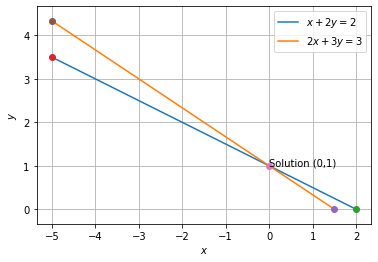
\includegraphics[width=\columnwidth]{a_2.png}
\caption{Lines and their intersection denoting the solution}
\label{b}
\end{figure}

$\therefore$ The given system of equation is consistent with unique solution of,
$$\myvec{x\\y}=\myvec{0\\1}$$
\end{document}
